\documentclass[12pt]{article}
\usepackage[utf8]{inputenc}
\usepackage[english]{babel}
\usepackage{amsmath, amsthm, amssymb, amsfonts}
\allowdisplaybreaks

\usepackage[top = 3in, left = 1in, right = 1in]{geometry}
\usepackage{hyperref}
\hypersetup{
	colorlinks=true,
	linkcolor=blue,
	filecolor=magenta,      
	urlcolor=blue,
}
\usepackage{tcolorbox}
\usepackage{bm}

% FOR TIKZ
\usepackage{tikz}
\usetikzlibrary{arrows,arrows.meta, shapes.geometric}


% DEFINE NEW COMMANDS AND ENVIRONMENTS
\newcommand{\R}{\mathbb{R}}
\newcommand{\C}{\mathbb{C}}
\newcommand{\N}{\mathbb{N}}
\newcommand{\Q}{\mathbb{Q}}
\newcommand{\Z}{\mathbb{Z}}
\newcommand{\transpose}{\mathsf{T}}

\newcommand{\E}{\mathbb{E}}
\newcommand{\Var}{\mathbb{V}}



\newcommand{\HRule}{\rule{\linewidth}{0.5mm}} % Defines a new command for the horizontal lines, change thickness here


% DEFINE A PROBLEM Environment
\theoremstyle{definition}
\newtheorem*{prb}{Problem}
\newenvironment{problem}{
\begin{tcolorbox}[colback=blue!5!white,colframe=blue!75!black, parbox = true] \begin{prb}  }{\end{prb}\end{tcolorbox} }


\newenvironment{answer}{\textit{Solution: }\quad }{ \hfill \qedsymbol}



\begin{document}


% TITLE PAGE
%%%%%%%%%%%%%%%%%%%%%%%%%%%%%%%%%%%%%%%%%%%%%%%%%%%%%%
\begin{titlepage}
    
\centering
\textsc{\LARGE Indian Statistical Institute, Kolkata}\\[1.5cm] % Name of your university/college
\textsc{\Large Sample Surveys}\\[0.5cm] % Major heading such as course name
\textsc{\large Assignments in lieu of Semestral Examinations 2020}\\[0.5cm] % Minor heading such as course title

\HRule \\[0.4cm]
\large \textbf{Subhrajyoty Roy}\\
\large \textbf{Roll:  MB1911}\\
\HRule \\[1.5cm]
\normalsize \today

\end{titlepage}


\tableofcontents
\clearpage


% CONTENT FROM HERE
%%%%%%%%%%%%%%%%%%%%%%%%%%%%%%%%%%%%%%%%%%%%%%%%%%
\newgeometry{margin = 1in}

\section{Problem 1}

\begin{problem}
	The following figures relate to a group of $15$ households.
	\begin{center}
		\begin{tabular}{|l|l|l|}
			\hline
			Serial No. & HH Size & Expenditure last month (Rs.)  \\ \hline
			1 & 8 & 5470.35 \\ \hline
			2 & 6 & 2716.80 \\ \hline
			3& 5& 1873.75 \\ \hline
			4& 4& 1693.20\\ \hline
			5& 3& 1393.55\\ \hline
			6& 6& 2398.74 \\ \hline
			7& 2& 3153.35\\ \hline
			8& 5& 2708.75\\ \hline
			9& 7& 2873.60\\ \hline
			10& 6& 3775.80\\ \hline
			11& 8& 5027.25\\ \hline
			12& 3& 1175.28\\ \hline
			13& 4& 2952.15\\ \hline
			14& 2& 1032.27\\ \hline
			15& 2& 2075.41\\ \hline
		\end{tabular}
	\end{center}
	
	 Consider the above data as a population data. Estimate the average last month's h.h. expenditure in this area based on Durbin (1967)'s IPPS sampling scheme of size $n=2$ h.h.s. with h.h. size as size measure. In addition give the estimates of standard error, CV and 95\% CI of  $\bar{Y}$.


	 Determine how the selection probability need to be modified for  Lahiri-Midzuno-Sen (1952)'s scheme to make the scheme as IPPS sampling scheme for $n=6$.
\end{problem}

\begin{answer}
	Let, $X_i$ be the size measure value of $i$-th household unit. Then, the size measure probabilities $p_i$'s would be given as, $p_i = \dfrac{X_i}{X}$, where $X = \sum_{i=1}^{15}X_i$. 

	From the table given in the question, we obtain $X = 71$, and the size measure probabilities can be easily obtained as;

	$$
	\begin{array}{lllll}
		0.11267606 &  0.08450704 & 0.07042254 & 0.05633803 & 0.04225352\\
		0.08450704 & 0.02816901 & 0.07042254 & 0.09859155 & 0.08450704\\
		0.11267606 & 0.04225352 & 0.05633803 & 0.02816901 & 0.02816901\\
	\end{array}
	$$

	Based on a random number table, a random two digit integer is chosen and is found to be equal to $43$. Considering the cumulative sum of the size measure values, the household $9$ is sampled as first unit, in accordance to a probability proportional sampling scheme.

	Now, based on Durbin's IPPS scheme, the second order sampling probabilities are obtained by the formula;

	$$P(j \mid i) = \dfrac{p_j\left[ \dfrac{1}{1 - 2p_i} + \dfrac{1}{1 - 2p_j} \right]}{1 + \sum_{i=1}^{N} \dfrac{p_i}{1 - 2p_i}}$$

	Based on the remaining $14$ households, except the unit $9$, we have the following revised size measure probabilities;

	$$
	\begin{array}{lllllll}
		0.13041071 & 0.09443330 & 0.07742659 & 0.06099140 & 0.04507499 & 0.09443330 & 0.02963090\\
		0.07742659 & 0.09443330 & 0.13041071 & 0.04507499 & 0.06099140 & 0.02963090 & 0.02963090\\
	\end{array}
	$$

	Similar to before, another probability proportional sampling is employed, and household $1$ is selected this time.

	Therefore, our sample of size $n = 2$, consists of the following:

	\begin{table}[h]
		\centering
		\begin{tabular}{|c|c|c|c|}
			\hline
			\textbf{Serial No.} & $p_i$ & $P(j \mid i)$ & \textbf{Expenditure last month}\\
			\hline
			9 & $0.09859155$ & - & $2873.60$\\
			1 & $0.11267606$ & $0.13041071$ & $5470.35$\\
			\hline
		\end{tabular}
	\end{table}

	Therefore, the estimate of average last month's household expenditure is;

	$$\widehat{\bar{Y}}_{HT} 
	= \dfrac{1}{N} \sum_{i \in s} \dfrac{y_i}{\pi_i} 
	= \dfrac{1}{N} \sum_{i \in s} \dfrac{y_i}{2p_i}
	= \dfrac{1}{30} \left( \dfrac{2873.60}{0.09859155} + \dfrac{5470.35}{0.11267606} \right)
	= \dfrac{77695.86875}{30}
	= 2589.86
	$$

	We also know that,

	$$\Var(\widehat{\bar{Y}}_{HT}) = \dfrac{1}{N^2}\left[\sum_{i=1}^{N} Y_i^2 \left( \dfrac{1 - \pi_i}{\pi_i} \right) + \sum_{i \neq j, 1}^{N} Y_iY_j\left( \dfrac{\pi_{ij} - \pi_i \pi_j}{\pi_i \pi_j} \right)\right]$$

	and since IPPS scheme is a fixed effective sample size preserving design, we have Yate's and Grundy's form of variance estimator as;

	$$\widehat{\Var}(\widehat{\bar{Y}}_{HT}) = \dfrac{1}{N^2} \left[\sum_{i\neq j \in s} \left( \dfrac{\pi_i \pi_j - \pi_{ij}}{\pi_{ij}} \right) \left( \dfrac{y_i}{\pi_i} - \dfrac{y_j}{\pi_j} \right)^2\right]$$

	In case of Durbin's IPPS scheme with $n = 2$, 

	$$\pi_{ij} = 2 \dfrac{p_i p_j \left[ \dfrac{1}{1 - 2p_i}  + \dfrac{1}{1 - 2p_j} \right]}{1 + \sum_{i=1}^{N} \dfrac{p_i}{1 - 2p_i} }$$

	which for the obtained samples $1$ and $9$-th household turns out to be; $\pi_{19} = 0.02571479$ after some calculation. We also have, $\pi_i = 2p_i$. Therefore, we obtain;

	\begin{align*}
		\widehat{\Var}(\widehat{Y}_{HT})
		& = \dfrac{1}{15^2} \left[\sum_{i\neq j \in s} \left( \dfrac{4p_i p_j - \pi_{ij}}{\pi_{ij}} \right) \left( \dfrac{y_i}{2p_i} - \dfrac{y_j}{2p_j} \right)^2 \right]\\
		& = \dfrac{1}{225} \left[ 0.7280184 \times 19402.84^2 \right]\\
		& = 1218121
	\end{align*}

	Therefore, the estimate of standard error is; $\widehat{SE}(\widehat{\bar{Y}}_{HT}) = \sqrt{1218121} \approx 1103.685$.

	Consequently, the estimate of CV can be obtained by the formula;
	$$\widehat{CV} = \dfrac{\widehat{SE}(\widehat{\bar{Y}}_{HT})}{\widehat{\bar{Y}}_{HT}} \times 100\% $$

	and the $95\%$ asymptotic confidence interval as;

	$$\left( \widehat{\bar{Y}}_{HT} - 1.96\widehat{SE}(\widehat{\bar{Y}}_{HT}), \widehat{\bar{Y}}_{HT} + 1.96\widehat{SE}(\widehat{\bar{Y}}_{HT}) \right)$$

	Therefore, the final estimates turn out to be as follows:

	\begin{align*}
		\widehat{\bar{Y}}_{HT} & = 2589.86 \text{ Rupees }\\
		\widehat{SE}(\widehat{\bar{Y}}_{HT}) & = 1103.685 \text{ Rupees}\\
		\widehat{CV} & = \dfrac{2589.86}{1103.685}\times 100\% = 42.61562\%\\
		95\% \text{ Confidence interval} & = 426.64 \text{ Rupees to }  4753.08 \text{ Rupees.}\\
	\end{align*}


	In case of Lahiri-Midzuno-Sen's scheme for IPPS sampling with $n = 6$, the new selection probabilities $p_i^\ast$ is obtained by the following modification over the usual selection probabilities $p_i = \dfrac{X_i}{X}$ values.

	$$p_i^\ast = \dfrac{n(N-1)}{N - n} p_i - \dfrac{n-1}{N-n}$$

	In the given problem, $N = 15$ and $n = 6$, therefore, the above formula becomes;

	$$p_i^\ast = \dfrac{28}{3} p_i - \dfrac{5}{9}$$

	However, such modification would result in some of $p_i^\ast$'s being negative, as for some the units in the population, the required condition $p_i \geq \dfrac{(n-1)}{n(N-1)}$ is not satisfied, and hence Lahiri-Midzuno-Sen's method cannot be applied.
\end{answer}




\section{Problem 2}

\begin{problem}
	Explain how the double sampling approach can be used to overcome the problem in stratified random sampling when the stratum preparation are not completely known.
\end{problem}

\begin{answer}
	Suppose we define the $h$-th stratum of a survey population of $N$ units, as the set of units bearing $y$-values in the range $(a_{h-1}, a_h)$ for $h = 1, 2, \dots H$. However, since the stratum preparation are not completely known in the sense that which units have $y$-values in which intervals are not known.

	To deal with this problem Double sampling approach can be used. 
	
	\begin{enumerate}
		\item Let a SRSWOR of $n_1$ units be taken and $y$-values of these selected units are collected.
		\item Based on the collected $y$-values, we distribute $n_1$ sampled units to $H$ predefined strata. Let $n_{1h}$ be the number of units falling in the $h$-th range $(a_{h-1}, a_h)$.
		\item Let independently across $H$ strata, for $h = 1, 2, \dots H$, SRSWOR of sizes $n_{2h}$ be drawn out of $n_{1h}$ units. 
	\end{enumerate}
	
	Then, the following estimator;

	$$\bar{y}_{st} = \sum_{h = 1}^{H}w_h \bar{y}_{2h}$$

	where $\bar{y}_{2h}$ be the sample mean for $h$-th stratum based on these $n_{2h}$ sampled units, and $w_{1h} = \dfrac{n_{1h}}{n_1}$.

	Let us denote $\E_1, \E_2, \E$ and $\Var_1, \Var_2, \Var$ as the expectation and variance operators with respect to sample selection initially, stratified sampling of $n_{2h}$ units out of them realized sets of $n_{1h}$ units for $h = 1, 2, \dots H$ and the overall sampling procedure.

	Firstly, we show that this estimator $\bar{y}_{st}$ is unbiased for the population mean $\bar{Y}$.

	Note that,

	\begin{align*}
		\E(\bar{y}_{st}) & = \E_1 \E_2 \left( \sum_{h = 1}^{H}w_h \bar{y}_{2h} \right)\\
		& = \E_1 \left( \sum_{h = 1}^{H} w_h \E_2 \left( \bar{y}_{2h} \right) \right)\\
		& = \E_1 \left( \sum_{h = 1}^{H} w_h \bar{y}_{1h} \right)\qquad \text{, since } \bar{y}_{2h} \text{ is SRSWOR mean of } h \text{-th stratum} \\
		& = \E_1 \left( \sum_{h = 1}^{H} \dfrac{n_{1h}}{n_1} \dfrac{1}{n_{1h}} \sum_{i = 1}^{n_{1h}} y_{hi} \right)\\
		& = \E_1 \left( \dfrac{1}{n_1} \sum_{h = 1}^{H} \sum_{i = 1}^{n_{1h}} y_{hi} \right)\\
		& = \E_1(\bar{y}_1) \\
		& = \bar{Y} \qquad \text{, since } \bar{y}_1  \text{ is again SRSWOR sample mean} \\
	\end{align*}
	
	Therefore, $\bar{y}_{st}$ is unbiased for population mean. 

	Now, note that, $\E_2(\bar{y}_{st}) = \bar{y}_1$, which is SRSWOR sample mean. 

	Hence, $\Var_1\E_2(\bar{y}_{st}) = \Var_1\left( \bar{y}_1 \right) = \left( \dfrac{1}{n_1} - \dfrac{1}{N}\right)S^2$.
	
	Also,

	\begin{align*}
		\Var_2\left( \bar{y}_{st} \right) & = \Var_2 \left( \sum_{h = 1}^{H}w_h \bar{y}_{2h} \right)\\
		& = \sum_{h = 1}^{H} w_h^2 \Var_2(\bar{y}_{2h})\\
		& = \sum_{h = 1}^{H} \dfrac{n_{1h}^2}{n_1^2} \left( \dfrac{1}{n_{2h}} - \dfrac{1}{n_{1h}} \right) \dfrac{1}{n_{2h} - 1} \sum_{i = 1}^{n_{1h}} \left(y_{hi} - \bar{y}_{1h}\right)^2\\
		& = \sum_{h = 1}^{H} \dfrac{n_{1h}^2}{n_1^2} \left( \dfrac{1}{n_{2h}} - \dfrac{1}{n_{1h}} \right) s_{1h}^2 \text{, where } s_{1h}^2 \text{ is the quantity it is replacing}\\
		& = \sum_{h = 1}^{H} \dfrac{n_{1h}}{n_1} \left( \dfrac{1}{n_{2h} / n_{1h}} - 1 \right) s_{1h}^2\\
		& = \sum_{h = 1}^{H} \dfrac{n_{1h}}{n_1} \left( \dfrac{1}{\gamma_h} - 1 \right) s_{1h}^2\\
	\end{align*}

	where $\gamma_h = \dfrac{n_{2h}}{n_{1h}}$ is the sampling fraction for $h$-th stratum.

	Now let $\E_{1c}$ denotes the expectation conditioned on the fixed configuration of $\mathbf{n}_1 = \left(n_{11}, n_{12}, \dots n_{1H}\right)$, and $\E_{1u}$ denotes the expectation operator over the variability inherent in the sampling of the 1st phase.

	So, 

	$$\E_{1c}(s_{1h}^2) = \E_{1c}\left( \dfrac{1}{n_{2h} - 1} \sum_{i = 1}^{n_{1h}} \left(y_{hi} - \bar{y}_{1h}\right)^2 \mid \mathbf{n}_1 \right) = S_h^2$$

	since, $s_{1h}^2$ is the unbiased estimator of the variance of SRSWOR estimator of mean. Also, $\E_{1u}(w_h) = \E_{1u}\left( \dfrac{n_{1h}}{n_1} \right) = \dfrac{N_h}{N} = W_h$.

	So, we have;
	
	\begin{equation*}
		\E_1(w_h s_{1h}^2) = \E_{1u}(w_h \E_{1c} (s_{1h}^2)) = S_h^2 \E_{1u}(w_h) = W_hS_h^2
	\end{equation*}

	Hence, 
	\begin{align*}
		\Var(\bar{y}_{st}) 
		& = \E_1\Var_2(\bar{y}_{st}) + \E_2\Var_1(\bar{y}_{st})\\
		& = \left( \dfrac{1}{n_1} - \dfrac{1}{N} \right)S^2 + \dfrac{1}{n_1} \sum_{h=1}^{H} \left(\dfrac{1}{\gamma_h} - 1\right) W_h S_h^2
	\end{align*}

\end{answer}




\section{Problem 3}

\begin{problem}
	Explain how non-response situation in an SRSWR surveys can be handled by Politz and Simmon's `at-home-probability' technique without additional attempt of recovering data. 
\end{problem}

\begin{answer}
	Pollitz and Simmons (1949, 1950, JASA) have introducted the method of using the "probabilities at-home" to estimate the population mean of a variable of interest, in a non-response situation. 

	In this scheme, The interviewer makes only one call at each sampled household, the time of call being random within the interviewing hours. If the eligible respondent is available
	at the house, the information of the actual response variable $y$ is collected and it is also asked whether the respondent was at home on the previous six days at the same time. This information is used to estimate $p$, the probability of being at home.

	Assuming an SRSWR sampling scheme, let us consider the following estimate of $y_i$, the value of the response variable for $i$-th household;

	$$\widehat{y_i} = \begin{cases}
		\dfrac{y_i}{\widehat{p_i}} & \text{ if respondent of } i\text{-th household is available}\\
		0 & \text{ otherwise}
	\end{cases}$$

	where $\widehat{p_i} = j/7$, where $j$ being the number of days (six days before and the interviewing day) when the respondent was available at home at the same time of the day. In general, we can consider $\widehat{p_i} = j/s$, where $(s-1)$ is the number of days for which the "at-home" responsess (i.e. whether the respondent was "at-home" on that day) is collected.

	For an unit $i$ for which the respondent was available, we have the expectation of $\widehat{y_i}$ conditioned on the fact that respondent is sampled and available at home;

	\begin{align*}
		\E_c(\widehat{y_i})
		& = \sum_{j = 1}^{s} \dfrac{y_i}{j/s} \binom{s-1}{j-1} p_i^{j-1} (1 - p_i)^{s-j}, \\
		& \qquad \qquad \text{since leaving interviewing date, the number of days respondent}\\
		& \qquad \qquad \text{was at-home follows binomial distribution}\\
		& \qquad \qquad \text{and let } p_i \text{ be the at-home probability for respondent } i;\\ 
		& = y_i \sum_{j = 1}^{s} \dfrac{s}{j} \binom{s-1}{j-1} p_i^{j-1} (1 - p_i)^{s-j}\\
		& = y_i \sum_{j = 1}^{s} \binom{s}{j} p_i^{j-1} (1 - p_i)^{s-j}\\
		& = \dfrac{y_i}{p_i} \left[ 1 - q_i^s \right]\\
		& \qquad \qquad \text{ where } q_i = (1 - p_i)\\
	\end{align*}

	Now, taking into account that the probability of availability of household $i$ is $p_i$ and Probability of selecting that household is $1/N$, the unconditional expectation becomes;

	\begin{align*}
		\E_u(\widehat{y_i})
		& = \sum_{i = 1}^{N} \dfrac{Y_i (1 - q_i^s)}{p_i} \times p_i \times \dfrac{1}{N}\\
    	& = \dfrac{1}{N} \sum_{i = 1}^{N} \left( Y_i - Y_i q_i^s \right)\\
    	& = \overline{Y} - \dfrac{1}{N} \sum_{i=1}^{N} Y_i q_i^s
	\end{align*}

	Finally, we can use the estimator as suggested by Pollitz and Simmons, 

	$$\widehat{\overline{Y_{PS}}} = \dfrac{1}{n} \sum_{i=1}^{n} y_i$$

	which has the expectation as $\E(\widehat{\overline{Y_{PS}}}) = \overline{Y} - \dfrac{1}{N} \sum_{i=1}^{N} Y_i q_i^s$, which is a biased estimator with bias being equal to $-\dfrac{1}{N} \sum_{i=1}^{N} Y_i q_i^s$, which is very small if $s$ is large, as then $q_i^s$ would be close to 0.	

\end{answer}


\section{Problem 4}

\begin{problem}
	Suppose $y$ is a real valued variable relating to a stigmatizing characteristics like expenses on treatment of AIDS, gain or loss through gambling during last month, money earned or spent in dubious means, etc. Let $Y_i$ denote the value of the $i_{th}$ person, $i=1,2,\ldots,N$. The problem is to estimate the population mean $\bar{Y} = \sum_{i=1}^N Y_i / N $. 

	Suppose $n$ persons are selected by using a sampling scheme which has the properties that $\pi_i > 0, \forall i = 1,2,\ldots, N$ and $\pi_{ij} > 0 , \forall i \neq j, i,j \in U=\{1,2,\ldots,N \}$. 

	To gather randomized response from a sampled person, suppose an investigator approaches with a box of cards marked (i) `True $y$ value' with $C$ as their proportion or (ii) marked $x_1, \ldots, x_j, \ldots, x_M$ with respective proportions $q_1, \ldots, q_j, \ldots, q_M$, such that $C + \sum_{j=1}^M q_j = 1$. The device thus produces the RR for $i_{th}$ person as;

	$$
	z_i = \begin{cases}
		y_i & \text{if `True y value' card appears}\\
		x_j & \text{ if } x_j \text{ card appears}
	\end{cases}
	$$
\end{problem}
 
Based on the  RRs gathered using such box, 

\begin{enumerate}
	\item[(a)] Obtain an unbiased estimator of $\bar{Y}$
	\item[(b)] Also obtain an unbiased variance estimator of (a).
\end{enumerate}

\begin{answer}
	Let, $\E_R, \Var_R$ be the expectation and variance operator with respect to the randomization device as given in the problem. Let, $\E_p$ and $\Var_p$ denote the expectation and variance operator with respect to the specific sampling scheme employed.

	Now, we have;

	\begin{align*}
		\E_R(z_i) & = C y_i + \sum_{j=1}^{M} q_jx_j\\
		\therefore \qquad \E_R(r_i) & = y_i \qquad \text{ where } r_i = \dfrac{z_i - \sum_{j=1}^{M} q_jx_j }{C}
	\end{align*}

	Clearly, $r_i$ can be regarded as a sample statistic as $z_i, q_j, x_j, C$ are all known quantity by the randomization device.

	Since, in the specific sampling scheme employed, we have first order inclusion probability, $\pi_i > 0$ for all $i = 1, 2, \dots N$, hence similar to Horvitz Thompson's estimator, we may consider,

	$$t_{HTR} = t_{HTR}(s, \bm{R}) = 
	\dfrac{1}{N} \sum_{i \in s} \dfrac{r_i}{\pi_i}$$

	where $\bm{R} = (r_1, r_2, \dots r_N)$ be randomized responses.
	
	Then,
	\begin{align*}
		\E(t_{HTR})
		& = \E_p \E_R \left( \dfrac{1}{N} \sum_{i \in s} \dfrac{r_i}{\pi_i} \right)\\
		& = \E_p \left[ \dfrac{1}{N} \sum_{i \in s} \dfrac{\E_R(r_i)}{\pi_i} \right]\\
		& = \E_p \left[ \dfrac{1}{N} \sum_{i \in s} \dfrac{y_i}{\pi_i} \right] \\
		& = \dfrac{1}{N} Y \qquad \text{, as HT estimator is unbiased for population total } Y = \sum_{i=1}^{N}Y_i\\
		& = \bar{Y}
	\end{align*}

	Therefore, $t_{HTR}$ is an unbiased estimator of $\bar{Y}$. \textbf{This solves part (a)}.

	Now, turning our attention to $r_i$,

	\begin{align*}
		\Var_R(r_i)
		& = \dfrac{1}{C^2} \Var_R(z_i) \qquad \text{, since } \sum_{j=1}^{M} q_jx_j \text{ is constant}\\
		& = \dfrac{1}{C^2} \left[ \E_R(z_i^2) - \E_R(z_i)^2 \right]\\
		& = \dfrac{1}{C^2} \left[ y_i^2 C + \sum_{j=1}^{M} q_jx_j^2 - \left( Cy_i + \sum_{j=1}^{M}q_jx_j \right)^2 \right]\\
		& = \dfrac{1}{C^2} \left[ C(1-C)y_i^2 - 2Cy_i \sum_{j=1}^{M}q_jx_j + \sum_{j=1}^{M}q_jx_j^2 - \left( \sum_{j=1}^{M}q_jx_j \right)^2 \right]\\
		& = \alpha y_i^2 + \beta y_i + \gamma
	\end{align*}

	where,

	\begin{align*}
		\alpha & = \dfrac{(1-C)}{C}\\
		\beta & = \dfrac{\sum_{j=1}^{M}q_jx_j}{C}\\
		\gamma & = \dfrac{1}{C^2} \left[ \sum_{j=1}^{M}q_jx_j^2 - \left( \sum_{j=1}^{M}q_jx_j \right)^2 \right] 
	\end{align*}

	Let us denote $\Var_R(r_i) = (\alpha y_i^2 + \beta y_i + \gamma) = V_i$.

	Now, considering the variance of the estimator $t_{HTR}$, we have;

	\begin{align*}
		\Var(t_{HTR})
		& = \E_p \Var_R(t_{HTR}) + \Var_p \E_R(t_{HTR})\\
		& = \E_p \left(\dfrac{1}{N^2} \Var_R \left[ \sum_{i \in s} \dfrac{r_i}{\pi_i} \right] \right) + \Var_p \left[ \dfrac{1}{N} \sum_{i \in s} \dfrac{y_i}{\pi_i} \right], \qquad \text{ since } \E_R(r_i) = \dfrac{1}{N} \sum_{i \in s} \dfrac{y_i}{\pi_i}\\
		& = \dfrac{1}{N^2} \E_p \left[ \sum_{i \in s} \dfrac{V_i}{\pi_i^2} \right] + V_{HT}, \qquad \text{ since } r_i\text{'s are independent} \\
		& \qquad \qquad \text{ where } V_{HT} \text{ is the variance of Horvitz Thompson estimator}\\
		& = \dfrac{1}{N^2} \sum_{i = 1}^{N} \dfrac{V_i}{\pi_i^2} \E_p(\bm{1}_{si}) + V_{HT}, \qquad \text{ where } \bm{1}_{si} \text{ takes value 1 if } i \in s \text{, 0 otherwise}\\
		& = \dfrac{1}{N^2} \sum_{i = 1}^{N} \dfrac{V_i}{\pi_i} + V_{HT}, \text{ since } \E_p(\bm{1}_{si}) = \pi_i
	\end{align*}

	We also know that,

	$$V_{HT} = \dfrac{1}{N^2} \left[\sum_{i = 1}^{N} Y_i^2 \left(\dfrac{1 - \pi_i}{\pi_i}\right) + \sum_{i \neq j} Y_i Y_j \left(\dfrac{\pi_{ij} - \pi_i \pi_j}{\pi_i \pi_j}\right)\right] $$

	from the formula of variance of Horvitz Thompson estimator.

	Now, let us consider the quantity;

	$$v_i = \dfrac{\alpha r_i^2 + \beta r_i + \gamma}{(1 + \alpha)}$$

	where $\alpha, \beta, \gamma$ are known quantities as mentioned before.

	Then,

	\begin{align*}
		\E_R(v_i)
		& = \dfrac{1}{(1 + \alpha)} \left[ \alpha \E_R(r_i^2) + \beta \E_R(r_i) + \gamma \right]\\
		& = \dfrac{1}{(1 + \alpha)} \left[ \alpha (\Var_R(r_i^2) + \E_R(r_i)^2) + \beta \E_R(r_i) + \gamma \right]\\
		& = \dfrac{1}{(1 + \alpha)} \left[ \alpha V_i + \alpha y_i^2 + \beta y_i + \gamma \right]\\
		& = \dfrac{1}{(1 + \alpha)} V_i (1 + \alpha)\\
		& = V_i
	\end{align*}

	Assuming, 

	$$\alpha_i = \sum_{j=1}^{N} \left( \dfrac{\pi_{ij} - \pi_i \pi_j}{\pi_i} \right)$$

	We consider the following expression;

	\begin{align*}
		& \E\left[ \sum_{i \in s} \dfrac{v_i}{\pi_i} +  \sum_{i \in s} \alpha_i \dfrac{r_i^2}{\pi_i^2} + \sum_{i < j \in s} \left( \dfrac{\pi_i \pi_j - \pi_{ij}}{\pi_{ij}} \right) \left( \dfrac{r_i}{\pi_i} - \dfrac{r_j}{\pi_j} \right)^2 \right]\\
		= \quad & \E_p \E_R \left[ \sum_{i \in s} \dfrac{v_i}{\pi_i} + \sum_{i \in s} \alpha_i \dfrac{r_i^2}{\pi_i^2} + \sum_{i < j \in s} \left( \dfrac{\pi_i \pi_j - \pi_{ij}}{\pi_{ij}} \right) \left( \dfrac{r_i}{\pi_i} - \dfrac{r_j}{\pi_j} \right)^2 \right] \\
		= \quad & \E_p \left[ \sum_{i \in s} \dfrac{V_i}{\pi_i} \right] + \E_p \left[ \sum_{i \in s} \alpha_i \dfrac{\E_R(r_i^2)}{\pi_i^2} \right] + \E_p \left[ \sum_{i < j \in s} \left( \dfrac{\pi_i \pi_j - \pi_{ij}}{\pi_{ij}} \right) \left[ \dfrac{\E_R(r_i^2)}{\pi_i^2} + \dfrac{\E_R(r_j^2)}{\pi_j^2} - 2\dfrac{\E_R(r_ir_j)}{\pi_i \pi_j} \right] \right] \\
		= \quad & \E_p \left[ \sum_{i \in s} \dfrac{V_i}{\pi_i} \right] + \E_p \left[ \sum_{i \in s} \alpha_i \dfrac{V_i + \E_R(r_i)^2}{\pi_i^2} \right] + \\
		& \qquad \qquad \qquad \E_p \left[ \dfrac{1}{2} \sum_{i \neq j \in s} \left( \dfrac{\pi_i \pi_j - \pi_{ij}}{\pi_{ij}} \right) \left[ 2\dfrac{\E_R(r_i^2)}{\pi_i^2} - 2\dfrac{\E_R(r_i)\E_R(r_j)}{\pi_i \pi_j} \right] \right] \\
		= \quad & \E_p \left[ \sum_{i \in s} \dfrac{V_i}{\pi_i} \right] + \E_p \left[ \sum_{i \in s}\alpha_i \dfrac{V_i + y_i^2}{\pi_i^2} \right] + \E_p \left[ \sum_{i \neq j \in s} \left( \dfrac{\pi_i \pi_j - \pi_{ij}}{\pi_{ij}} \right) \left[ \dfrac{V_i + y_i^2}{\pi_i^2} - \dfrac{y_i y_j}{\pi_i \pi_j} \right] \right]\\
	\end{align*}

	Now, treating each of these terms separately, we have the following:

	$$\E_p \left[ \sum_{i \in s} \dfrac{V_i}{\pi_i} \right]
	= \sum_{i=1}^{N} \dfrac{V_i}{\pi_i} \E_p(\bm{1}_{si})
	= \sum_{i=1}^{N} \dfrac{V_i}{\pi_i} \pi_i
	= \sum_{i=1}^{N} V_i$$

	Next,

	$$\E_p \left[ \sum_{i \in s}\alpha_i \dfrac{V_i + y_i^2}{\pi_i^2} \right]
	= \sum_{i=1}^{N} \alpha_i \dfrac{V_i + Y_i^2}{\pi_i^2} \E_p(\bm{1}_{si})
	= \sum_{i=1}^{N} \alpha_i \dfrac{V_i + Y_i^2}{\pi_i^2} \pi_i
	= \sum_{i=1}^{N} \alpha_i \dfrac{V_i + Y_i^2}{\pi_i}$$


	And,

	\begin{align*}
		& \E_p \left[ \sum_{i \neq j \in s} \left( \dfrac{\pi_i \pi_j - \pi_{ij}}{\pi_{ij}} \right) \left[ \dfrac{V_i + y_i^2}{\pi_i^2} - \dfrac{y_i y_j}{\pi_i \pi_j} \right] \right]\\
		= \quad & \sum_{i\neq j, 1}^{N} \left( \dfrac{\pi_i \pi_j - \pi_{ij}}{\pi_{ij}} \right) \left[ \dfrac{V_i + Y_i^2}{\pi_i^2} - \dfrac{Y_i Y_j}{\pi_i \pi_j} \right] \E_p(\bm{1}_{si} \bm{1}_{sj})\\
		= \quad & \sum_{i\neq j, 1}^{N} \left( \dfrac{\pi_i \pi_j - \pi_{ij}}{\pi_{ij}} \right) \left[ \dfrac{V_i + Y_i^2}{\pi_i^2} - \dfrac{Y_i Y_j}{\pi_i \pi_j} \right] \pi_{ij}\\
		= \quad & \sum_{i\neq j, 1}^{N} \left( \pi_i \pi_j - \pi_{ij} \right) \left[ \dfrac{V_i + Y_i^2}{\pi_i^2} - \dfrac{Y_i Y_j}{\pi_i \pi_j} \right]\\
		= \quad & \sum_{i = 1}^{N} \dfrac{V_i + Y_i^2}{\pi_i^2} \sum_{j \neq i}\left( \pi_i \pi_j - \pi_{ij} \right)  + \sum_{i\neq j, 1}^{N} \left( \pi_{ij} - \pi_i \pi_j  \right) \dfrac{Y_i Y_j}{\pi_i \pi_j} \\
		= \quad & \sum_{i = 1}^{N} \dfrac{V_i + Y_i^2}{\pi_i} \sum_{j \neq i}\left( \dfrac{\pi_i \pi_j - \pi_{ij}}{\pi_i} \right)  + \sum_{i\neq j, 1}^{N} \left( \pi_{ij} - \pi_i \pi_j  \right) \dfrac{Y_i Y_j}{\pi_i \pi_j} \\
		= \quad & \sum_{i = 1}^{N} \dfrac{V_i + Y_i^2}{\pi_i} \left[\sum_{j = 1}^{N} \left( \dfrac{\pi_i \pi_j - \pi_{ij}}{\pi_i} \right) - \left(\dfrac{\pi_i^2 - \pi_i}{\pi_i}\right) \right]  + \sum_{i\neq j, 1}^{N} \left( \pi_{ij} - \pi_i \pi_j  \right) \dfrac{Y_i Y_j}{\pi_i \pi_j} \\
		= \quad & \sum_{i = 1}^{N} \dfrac{V_i + Y_i^2}{\pi_i} \left[-\alpha_i - \left(\dfrac{\pi_i^2 - \pi_i}{\pi_i}\right) \right]  + \sum_{i\neq j, 1}^{N} \left( \pi_{ij} - \pi_i \pi_j  \right) \dfrac{Y_i Y_j}{\pi_i \pi_j} \\
	\end{align*}

	Therefore, summing these together, we obtain,

	\begin{align*}
		& \E\left[ \sum_{i \in s} \dfrac{v_i}{\pi_i} +  \sum_{i \in s} \alpha_i \dfrac{r_i^2}{\pi_i^2} + \sum_{i < j \in s} \left( \dfrac{\pi_i \pi_j - \pi_{ij}}{\pi_{ij}} \right) \left( \dfrac{r_i}{\pi_i} - \dfrac{r_j}{\pi_j} \right)^2 \right]\\
		= \quad & \sum_{i=1}^{N} V_i - \sum_{i=1}^{N} V_i \left( \dfrac{\pi_i - 1}{\pi_i} \right) + \sum_{i = 1}^{N} Y_i^2 \left(\dfrac{1 - \pi_i}{\pi_i}\right) + \sum_{i \neq j} Y_i Y_j \left(\dfrac{\pi_{ij} - \pi_i \pi_j}{\pi_i \pi_j}\right)\\
		= \quad & \sum_{i=1}^{N} \dfrac{V_i}{\pi_i} + N^2 \times V_{HT}
	\end{align*}

	Hence,

	$$\widehat{\Var(t_{HTR})} = \dfrac{1}{N^2} \left[ \sum_{i \in s} \dfrac{v_i}{\pi_i} +  \sum_{i \in s} \alpha_i \dfrac{r_i^2}{\pi_i^2} + \sum_{i < j \in s} \left( \dfrac{\pi_i \pi_j - \pi_{ij}}{\pi_{ij}} \right) \left( \dfrac{r_i}{\pi_i} - \dfrac{r_j}{\pi_j} \right)^2 \right] $$

	\textbf{This completes the solution to part (b).}
	
\end{answer}









\section{Problem 5}

\begin{problem}
	Define protection of privacy measure in estimating a sensitive population proportion based on SRSWR of respondents and by using RRT that produces either yes or no response. 

	By using illustration of Warner (1965)'s RR model, show that as the privacy is protected more and more the efficiency in estimation goes on declining.
\end{problem}


\begin{answer}
	Many RRT produces either ``yes i.e. match" or ``no i.e. not match" response from a pool of respondents chosen by SRSWR schemes in order to effectively estimate the population proportion relating to a sensitive attribute.
	
	Let, $A$ be the set of the population having the sensitive attribute, and $P(A) = \theta$. Then, $P(A^c) = (1 - \theta)$. Also assume, $P(\text{Yes} \mid A) = a$ and $P(\text{No} \mid A^c) = b$, where this $a$ and $b$ depends on the particular RR scheme.

	Now, using Bayes theorem it follows that;

	\begin{align*}
		P(A \mid \text{Yes}) 
		& = \dfrac{P(A) P(\text{Yes}\mid A) }{P(A) P(\text{Yes}\mid A) + P(A^c) P(\text{Yes}\mid A^c)}\\
		& = \dfrac{\theta a}{\theta a + (1-\theta) (1-b)}
	\end{align*}
	
	If $P(A \mid \text{Yes}) > P(A)$, then a person may hesitate to give a ``Yes" response because he / she may perceive this response to enhance his / her being inferred to bear $A$ rather than $A^c$.
	
	Similarly,
	
	\begin{align*}
		P(A^c \mid \text{No}) 
		& = \dfrac{P(A^c) P(\text{No}\mid A^c) }{P(A) P(\text{No}\mid A) + P(A^c) P(\text{No}\mid A^c)}\\
		& = \dfrac{(1 - \theta) b}{\theta (1-a) + (1-\theta) b}
	\end{align*}
	
	Now if $P(A^c \mid \text{No}) < (1-\theta)$, then ``No" answer may appear as a threat to the respondent's privacy.

	For this reason, the quantity,
    $$J(R) = \dfrac{P(A\mid R)/\theta}{P(A^c \mid R)/(1-\theta)}$$
    is taken as a \textbf{Measure of Jeopardy} in pronouncing a RR as $R$(``Yes or ``No") by a respondent, where $P(A\mid R)$ and $P(A^c\mid R)$ are probabilities of ``revealing" one's true feature being $A$ or $A^c$, conditional on their response $R$. The ideal value of $J(R)$, whether $R$ is either ``Yes" or ``No", which protects a respondent's identity is unity. The farther it is away from unity the less the response $R$ protects one's privacy.

	Now, in case of Warner's (1965) RR model, 

	\begin{align*}
		P(A \mid \text{Yes}) 
		& = \dfrac{P(A) P(\text{Yes}\mid A) }{ P(A) P(\text{Yes}\mid A) + P(A^c) P(\text{Yes}\mid A^c) }\\
		& = \dfrac{\theta p}{\theta p + (1-\theta) (1-p)}\\
		& = \dfrac{\theta p}{ \theta p + (1 - \theta) - p + \theta p }\\
		& = \dfrac{\theta p}{(1 - p) + (2p - 1)\theta}
	\end{align*}
	
	Clearly, $P(A \mid \text{Yes}) = \theta$, if and only if, $p = 1/2$. 

	However, for Warner's model, the variance of the estimator for SRSWR sampling scheme for the respondents is given as;

	$$\Var(\widehat{\theta}_A) = \dfrac{\lambda (1 - \lambda)}{n(2p - 1)^2}$$

	where $\lambda$ is the true proportion of people saying ``yes i.e. match'' and $n$ is the SRSWR sample size. Clearly, as $\vert p - 1/2 \vert \rightarrow 0$, the variance $\Var(\widehat{\theta}_A) \rightarrow \infty$. Also, for Warner's scheme the value $p = 1/2$ is not permissible. Therefore, as privacy is protected more and more, for Warner's scheme that would require $p \rightarrow 1/2$, and then the efficiency in estimation goes on declining as variance of the estimator increases constantly.
\end{answer}

\vspace*{1in}

\begin{center}
	{\Large\textit{Thank you}}
	\vspace*{0.25in}\\
	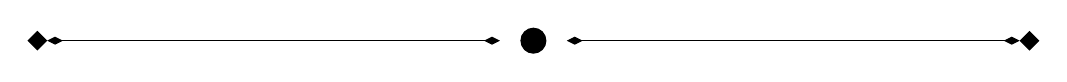
\begin{tikzpicture}[scale = 3]
		\node (a) at (0,0) {};
		\node (b) at (2,0) {};
		\draw[fill] (2.1, 0) circle (1.5pt);
		\node[draw, diamond, fill = black, scale = 0.5] at (0,0) {};
		\node (d) at (2.2,0) {};
		\node (e) at (4.2,0) {};
		\node[draw, diamond, fill = black, scale = 0.5] at (4.2,0) {};
		\draw [{Diamond}-{Diamond}] (a.east) -- (b.west);
		\draw [{Diamond}-{Diamond}] (d.east) -- (e.west);
	\end{tikzpicture}
\end{center}



\end{document}

